\documentclass{beamer}
\usepackage{xcolor}
\definecolor{olive}{rgb}{0.3, 0.4, .1}
\definecolor{fore}{RGB}{249,242,215}
\definecolor{back}{RGB}{51,51,51}
\definecolor{title}{RGB}{255,0,90}
\definecolor{dgreen}{rgb}{0.,0.6,0.}
\definecolor{gold}{rgb}{1.,0.84,0.}
\definecolor{JungleGreen}{cmyk}{0.99,0,0.52,0}
\definecolor{BlueGreen}{cmyk}{0.85,0,0.33,0}
\definecolor{RawSienna}{cmyk}{0,0.72,1,0.45}
\definecolor{Magenta}{cmyk}{0,1,0,0}
\newcommand{\blue}[1]{\textcolor{blue}{#1}}
\newcommand{\green}[1]{\textcolor{green}{#1}}
\newcommand{\dgreen}[1]{\textcolor{dgreen}{#1}}
\newcommand{\red}[1]{\textcolor{red}{#1}}
\newcommand{\purple}[1]{\textcolor{purple}{#1}}
\newcommand{\olive}[1]{\textcolor{olive}{#1}}

\newcommand{\cL}{\mathcal{L}}
\newcommand{\cO}{\mathcal{O}}

\newcommand{\bbQ}{\mathbb{Q}}
\newcommand{\bbZ}{\mathbb{Z}}

\newcommand{\Tr}{\mathrm{Tr}}
\newcommand{\TrKQ}{\mathrm{Tr}_{K/\mathbb{Q}}}
\newcommand{\NKQ}{\mathrm{N}_{K/\mathbb{Q}}}
\newcommand{\cOL}{\mathcal{O}^{\mathcal{L}}}
\newcommand{\cLV}{\mathcal{L}^{\vee}}
\newcommand{\vb}{\vec{b}}
\newcommand{\vbV}{\vec{b}^{\vee}}
% \usepackage{beamerthemesplit} // Activate for custom appearance

\title{Algebraically Structured LWE, Revisited}
\subtitle{Chris Peikert, Zachary Pepin}
\author{Yuncong Zhang}
\date{May 22, 2020}

\begin{document}

\frame{\titlepage}

\frame{\frametitle{Outline}\tableofcontents}

\section{Introduction}
\frame
{
  \frametitle{Background}
  Regev proposed the \blue{original LWE} [Reg09]

  \begin{itemize}
  	\item Average-case to worst-case security
  	\item Impractical efficiency
  \end{itemize}

  \blue{Structured LWE}s are LWEs with special structure on matrix $A$
  \begin{figure}[ht!]
  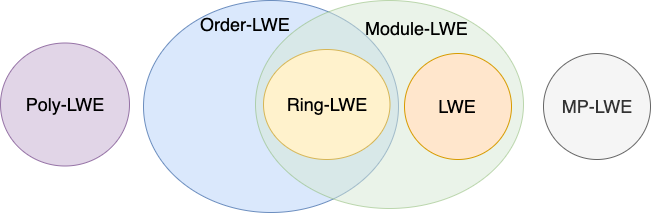
\includegraphics[width=0.5\textwidth]{files/Structured-LWE.png}
  \end{figure}

  \dgreen{Advantage: improved efficiency}\\
  \red{Disadvantages: complex security reduction}

}

\frame
{
  \frametitle{Contribution of this Paper}
  \begin{itemize}
  	\item A framework that encompasses \blue{ALL} structured LWE
  	\begin{figure}[ht!]
  	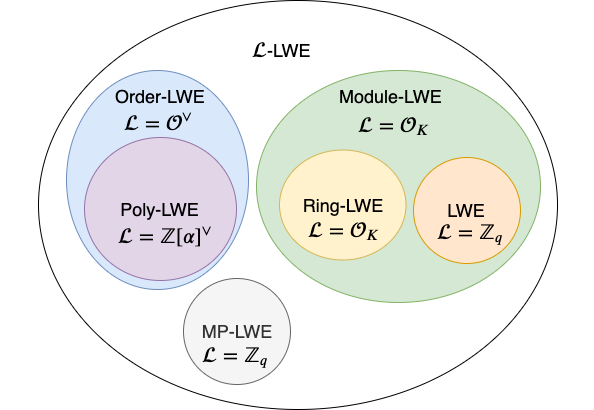
\includegraphics[width=0.5\textwidth]{files/L-LWE.png}
  	\end{figure}

  	\item Use this framework to give much \dgreen{simpler}, \dgreen{more general}, and \dgreen{tighter} reductions from Ring-LWE to other algebraic LWE variants
  	\begin{figure}[ht!]
  	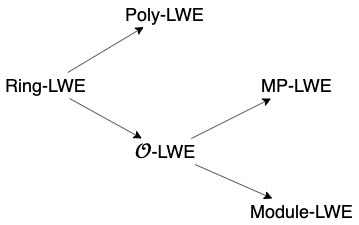
\includegraphics[width=0.5\textwidth]{files/LWE-Reductions.png}
  	\end{figure}

  \end{itemize}
}

\frame
{
  \frametitle{Algebraic Definitions}
  Let $K$ be a \blue{field extension} of $\bbQ$
  \begin{itemize}
  	\item Let degree-$d$ polynomial $f(x)\in\bbQ[X]$ \red{irreducible} over $\bbQ$
  	\item Let $\alpha\notin\bbQ$ be a \dgreen{root} of $f(x)$
  	\item $K=\bbQ(\alpha)$ is the \blue{minimal field} that contains $\alpha$
  \end{itemize}

  \noindent\rule{6cm}{0.4pt}\\
  Example:
  \begin{itemize}
  	\item $f(x)=x^2-2$ is irreducible over $\bbQ$
  	\item $\sqrt{2}\notin\bbQ$ is a root of $f(x)$
  	\item $K=\bbQ(\sqrt{2})=\{a+b\sqrt{2}\}_{a,b\in\bbQ}$
  \end{itemize}
}

\frame
{
  \frametitle{Algebraic Definitions}
  Given a \blue{basis} $\vec{b}=(b_1,b_2,\cdots,b_d)\in K$, $K$ is isomorphic to a $d$-dimensional \dgreen{vector space} over $\bbQ$
  \begin{itemize}
  	\item $(1,\sqrt{2})$ is a basis of $\bbQ(\sqrt{2})$
  \end{itemize}

  \noindent\rule{6cm}{0.4pt}\\
  For any $x\in K$, $x$ is identified with a \blue{map} $\phi_x:K\to K$ that is \olive{multiplication by} $x$
  \begin{itemize}
  	\item $\phi_x(y)=x\cdot y$
  	\item $\phi_x$ is linear, \blue{given a basis} $\vec{b}$, $\phi_x$ is \dgreen{identified with a matrix} $M_x$
  	\item For \blue{different} basis, $M_x$ \blue{varies}, but $\Tr(M_x)$ and $\det(M_x)$ are \dgreen{invariant}
  	\item Therefore, $\TrKQ(x):=\Tr(M_x)$ and $\NKQ(x):=\det(M_x)$, called the \blue{trace} and \blue{norm} of $x$, are \dgreen{well defined}
  \end{itemize}
}

\frame
{
  \frametitle{Algebraic Definitions}
  A \blue{lattice} $\cL\subseteq K$ is a \dgreen{discrete}, \dgreen{additive subgroup} of $K$

  \noindent\rule{6cm}{0.4pt}\\
  An \blue{Order} $\cO\subseteq K$ is \blue{both} a \dgreen{lattice} and a \dgreen{subring with unity} in $K$

  \noindent\rule{6cm}{0.4pt}\\
  \begin{itemize}
  	\item The \blue{ring of integers} $\cO_K$ is the \olive{maximal order} in $K$
  	\item The \blue{coefficient ring} of $\cL$ is $\cOL:=\{x\in K:x\cL\subseteq\cL\}$ which is \dgreen{also an order} of $K$
  \end{itemize}

  \noindent\rule{6cm}{0.4pt}\\
  An $n$-dimensional $\cL$ \blue{lattice} admits a \dgreen{$\bbZ$-basis} $\vb=(b_1,\cdots,b_n)$ in $K$
  \begin{itemize}
  	\item The \blue{dual lattice} of $\cL$ is $\cLV:=\{x\in K:\TrKQ(x\cL)\subseteq\bbZ\}$
  	\item The \blue{dual basis} $\vbV:=(b_1^{\vee},\cdots,b_n^{\vee})$ where $\TrKQ(b_i\cdot b_j)=\delta_{ij}$ \dgreen{is a basis of} $\cLV$
  \end{itemize}
}

\section{$\cL$-LWE}
\frame
{
  \frametitle{$\cL$-LWE}

}

\section{Reductions}
\frame
{
  \frametitle{Reduction from $\cL$-LWE to $\cL'$-LWE}

}

\frame
{
  \frametitle{Reduction from $\cO$-LWE to MP-LWE}

}

\frame
{
  \frametitle{Reduction from $\cO'$-LWE to $\cO$-LWE$^k$}

}

\end{document}
